\chapter{Esettanulmány}

Ebben a fejezetben bemutatom az eszköz használatát egy példamodellen. Ez a modell a Gamma tutorial csomagjában lévő közlekedési lámpákat tartalmazó modelljének SysML-be átemelt változata. A példán ismertetése közben bemutatom a az eszköz által támogatott modellezési módszertant is.

\section{A példamodel}

A modell három komponensből áll (\ref{fig:Crossroads} ábra): két a lámpákat irányító (\emph{primary}, \emph{secondary}) és egy az ezeket szinkronban tartó \emph{Controller} komponensből. A rendszernek van két kimeneti portja amellyel a két közlekedési lámpa jelzéseit tudja változtatni és rendelkezik egy bemeneti porttal amelyen keresztül a rendőrség \emph{Interrupted} ("Sárga villogó") állapotba tudja állítani a rendszert illetve vissza is tudja állítani a normál állapotba, ahol a piros - zöld - sárga jelzések váltakoznak a két lámpán mégpedig egymásnak ellentétesen.

\begin{figure}[!ht]
	\centering
	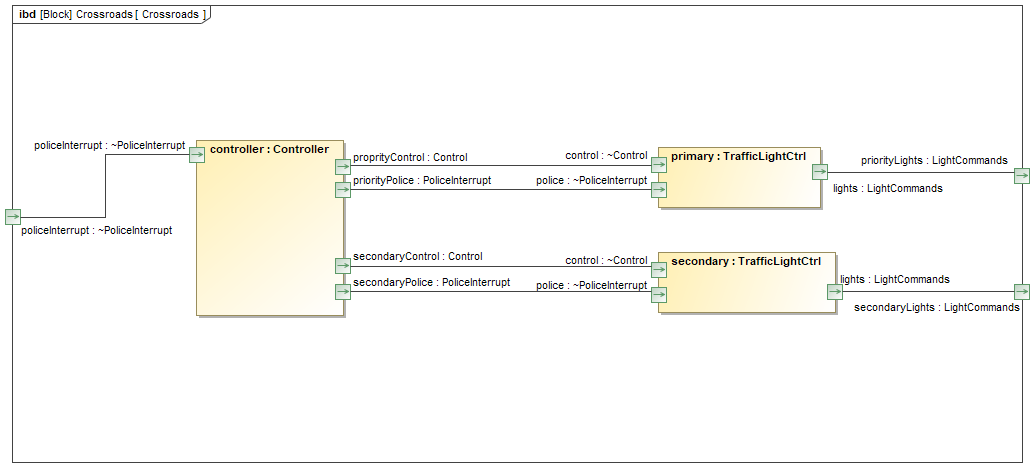
\includegraphics[width=15cm, keepaspectratio]{figures/contribution/Crossroads.png}
	\caption{Az útkereszteződés SysML modellje}
	\label{fig:Crossroads}
\end{figure}

A rendszer három interfészt definiál (\ref{fig:Interfaces} ábra): \emph{PoliceInterrupt}, \emph{Control}, \emph{LightCommands}. Ezek mindegyike \emph{Interface Block}ként kell, hogy megjelenjen a modellben, és minden az állapottérképeken használt \emph{Signal}hoz fel kell venni egy \emph{Flow Property}-t a megfelelő iránnyal. Jelen esetben ez a következőként jelenik meg. A \emph{Control} interfész tartalmaz egy \emph{Flow Property}-t \emph{out}, azaz kimenő iránnyal és egy 'toggle' nevű \emph{Signal}lal van tipizálva. Ez azért fontos mert az állapottérképen ezeket a \emph{Signal}okat kell majd használni. A \emph{LightCommands} négy kimenő \emph{Property}t tartalmaz. Ezek a \emph{displayNone}, \emph{displayRed}, \emph{displayGreed} és \emph{displayYellow} szignálokkal vannak tipizálva. A \emph{PoliceInterrupt} interfész csak egy \emph{Property}t tartalmaz \emph{out} iránnyal a \emph{police} szignálhoz.

\begin{figure}[!ht]
	\centering
	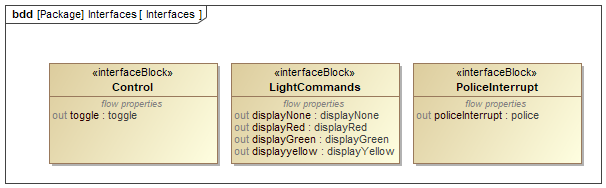
\includegraphics[width=15cm, keepaspectratio]{figures/contribution/Interfaces.png}
	\caption{Interfészek a modellben}
	\label{fig:Interfaces}
\end{figure}

Most, hogy már az interfészek és a portok le vannak modellezve el ezeket fel lehet használni az állapottérképek leírásához. A modell két állapottérképet definiál egyet a két lámpa controllerjéhez (\emph{LightCtr}-hez) és egyet a \emph{Controller}hez.

Tekintsük előbb a \emph{Controller} állapottérképére (\ref{fig:ControllerSM} ábra). Az állapotgép egy kompozit állapotból és ennek négy belső állapotából áll. \emph{Police Interrupt} hatására az állapotgép kilép a kompozit állapotból mindkét \emph{PoliceInterrupt} típusú portján küld egy-egy \emph{policeInterrupt} jelet, majd visszatér ugyan ebbe az állapotba. Amelyben a \emph{History State} miatt abból az állapotba kerül vissza amiben a kilépés előtt volt.

\begin{figure}[!ht]
	\centering
	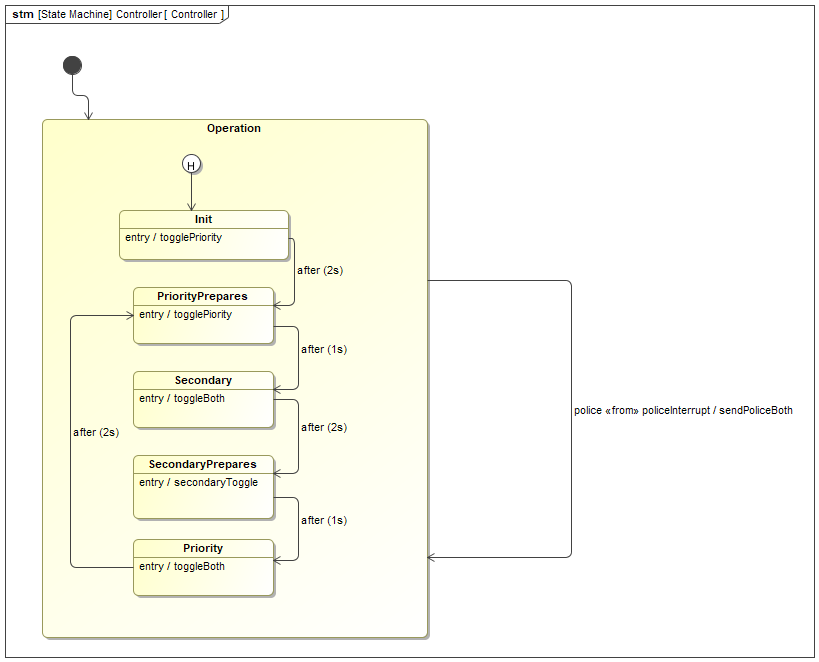
\includegraphics[width=12cm, keepaspectratio]{figures/contribution/ControllerSM.png}
	\caption{Controller állapotai}
	\label{fig:ControllerSM}
\end{figure}

Ami ennek az állapot átmenetnek a modellezése kapcsán izgalmas az \emph{Signal} küldésnek a módja. A plugin jelenlegi formájában ezt Activity diagrammal kell leírni \emph{Send Signal} akciók használatával. Ez jelen esetben egy két akciós \emph{Activity}t fog eredményezni, amelyben sorban a megfelelő portokon elküldésre kerülnek a szignálok (\ref{fig:activity} ábra).  A \emph{togglePriority}, \emph{secondaryToggle} és \emph{toggleBoth} \emph{entry action}ok hasonlóan vannak modellezve.

\begin{figure}[!ht]
	\centering
	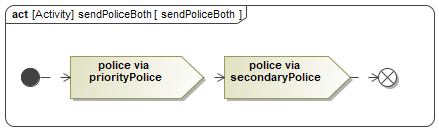
\includegraphics[width=12cm, keepaspectratio]{figures/contribution/sendPoliceBoth.png}
	\caption{\emph{Signal}ok küldése Activityel}
	\label{fig:activity}
\end{figure}

Amiről ennek az állapottérképnek a kapcsán még érdemes lehet beszélni ezek a bizonyos idő elteltével tüzelő átmenetek. Ezek a modellben \emph{Time Event}ként jelennek meg. Fontos hogy ezeknek a \emph{relative} attribútumát igazra kell állítani, hisz ez jelenti azt, hogy a forrás állapotba való belépéstől kell számítani az időt.

A teljesség kedvéért vizsgáljuk meg a másik állapottérképet is (\ref{fig:LightCtrlSM} ábra). Ez két kompozit állapotból áll. A \emph{Normál} a szokásos működést jelenti és a \emph{Red}, \emph{Green}, \emph{Yellow} állapotokból áll melyek a beérkező toggle szignálok hatására váltakoznak.
Az \emph{Interrupted} állapot a rendőrség által előidézett "sárga villogó" állapotot jelenti. Ebben a \emph{BlinkingYellow} és a \emph{Black} állapotok váltakoznak 500 milliszekundumonként.  

\begin{figure}[!ht]
	\centering
	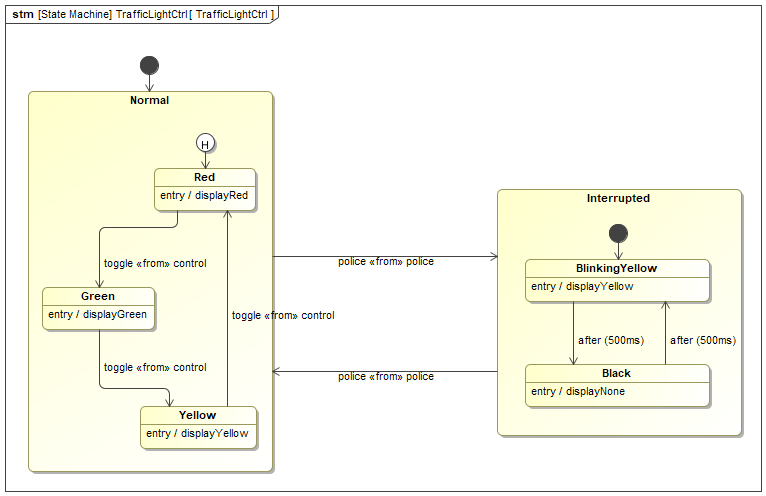
\includegraphics[width=12cm, keepaspectratio]{figures/contribution/TrafficLightCtrlSM.png}
	\caption{\emph{TrafficLightCtrl} állapottérképe}
	\label{fig:LightCtrlSM}
\end{figure}


\section{Transzformációk végrehajtása}

A modell összerakásánál egy dolog még nem lett lemodellezve, mégpedig, hogy melyik komponenst szemantikát szeretnénk alkalmazni. Jelen esetben a szinkron szemantikát szeretnénk. Ehhez jelen esetben elegendő a gyökér elem \emph{Block} sztereotípiáját a specifikusabb \emph{SynchronousCompositeComponent}re cserélni.
Most, hogy a komponens szemantika specifikálva van a modellek transzformálhatók és ellenőrizhetők.

Első lépésként létre kell hozni egy \emph{GammaWorkspace}t. Ez a modell elem fogja tárolni az ellenőrzés során szükséges adminisztrációs objektumokat. Azonban meg kell nevezni egy könyvtárat is a háttértáron amit ideiglenes fájlok tárolására fog a plugin használni. Ehhez egy \emph{Workspace Uri}t kell megadni ami egy abszolút elérési út egy tetszőleges könyvtárhoz. Az ellenőrizendő modellt a \emph{Target} mező megadásával lehet specifikálni.

\begin{figure}[!ht]
	\centering
	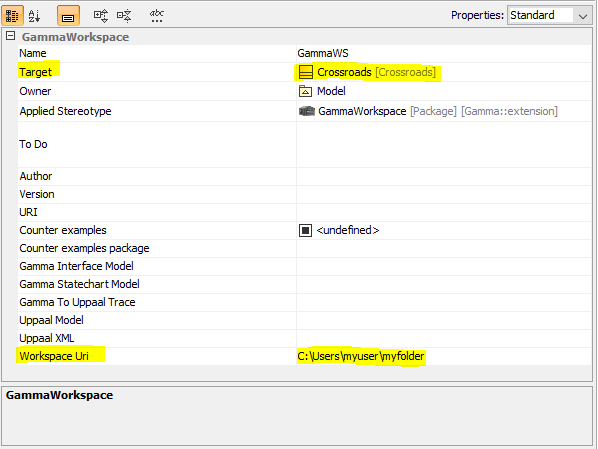
\includegraphics[width=7cm, keepaspectratio]{figures/contribution/GammaWS.png}
	\caption{\emph{GammaWorkspace} specifikációja}
	\label{fig:GammaWS}
\end{figure}


A kötelező mezők specifikálása után a \emph{Gamma Workspace}n nyitott gyorsmenüben a \emph{Gamma Transformation} menüpont alatt található akciók segítségével tudjuk a transzformációkat végrehajtani (\ref{fig:gamma-tra}). Az egymással függésben lévő lépések akkor válnak aktívvá, hogyha a bemenetük már előállt.

\begin{figure}[!ht]
	\centering
	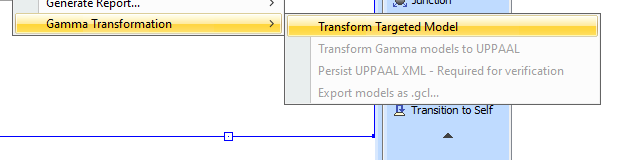
\includegraphics[width=10cm, keepaspectratio]{figures/contribution/GammaTransformation.png}
	\caption{Gyormenü elérése a transzformációkhoz}
	\label{fig:gamma-tra}
\end{figure}

Az akció végrehajtását követően két dolog történik. Először is megjelenik két \emph{GammaModel} sztereotípiával ellátott osztály elem, a transzformált interfészeknek és a komponenst modelleknek illetve állapotgépeknek. Másfelől a \emph{GammaWorkspace} \emph{Gamma Statechart Model} és a \emph{Gamma Interface Model} mezők ezekre fognak mutatni. A letranszformált modellek ezekhez a sztereotipizált osztályokhoz XMI formátumban kommentek formájában hozzá lesznek rendelve innen lehet őket \emph{EMF Resource}okba visszaolvasni amennyiben erre szükség van, így nem kell újra letranszformálni a modelleket.

Az osztályok belsejében továbbá létrejön jó pár \emph{property}. Ezek csomópont hivatkozások az XMI fájlok egyes elemeire. Belőlük pedig \emph{Trace} élek futnak melyek MagicDraw elemekre mutatnak. Ez az a visszakövethetőségi modell melynek segítségével tudjuk, hogy melyik Gamma elem milyen MagicDraw elemekből állt elő. Ezt \aref{fig:traces} ábra szemlélteti, ahol a \emph{Traced element} egy származtatott oszlop a \emph{Trace} élek cél elemei.

\begin{figure}[!ht]
	\centering
	\includegraphics[width=10cm, keepaspectratio]{figures/contribution/Traces.png}
	\caption{Elemek visszakövethetősége MagicDrawban (részlet)}
	\label{fig:traces}
\end{figure}

Következő lépés a az UPPAAL EMF speficikus modelljének előállítása  ez ehhez tartozó \emph{trace}kkel együtt amelyeket a Gamma majd a back-annotation előállításához használ majd. Ezeket a mostmár aktív "Transform models to UPPAAL" akció végrehajtásával tudjuk megtenni. Hasonlóan ez előbb szemléltetettekhez létrejön két sztereotipizált osztály egy az UPPAAL modellnek egy pedig az UPPAAL - Gamma \emph{traceknek}. A modellek ugyan úgy mint az előbb XMI formátumban az elemekhez lesznek kapcsolva. Ebben az esetben nem fognak \emph{property}k megjelenni hiszen ezek a modellek tulajdonképpen nem függnek a MagicDraw modelltől hanem funkcionálisan a Gamma részei.

Az eddigiekben nem volt szükség a háttértárra sorosítani, minden a MagicDraw modell belsejében került tárolásra. Azonban a következő lépés már használni fogja a behivatkozott könyvtárat is. Ez az utolsó lépés amit el kell végeznünk ahhoz, hogy olyan leírás álljon elő amit már az UPPAAL ellenőrzője be tud olvasni. Erre a \emph{Persist UPPAAL XML akció szolgál}. Ez szintén létrehoz egy sztereotipizált osztály elemet ez azonban már nem a \emph{GammaModel} hanem a \emph{GammaWorkspaceFile} sztereotípiát fogja megkapni. Ez utal arra, hogy ez egy külső hivatkozás (\ref{fig:gwsfinal} ábra).

\begin{figure}[!ht]
	\centering
	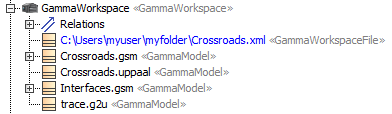
\includegraphics[width=10cm, keepaspectratio]{figures/contribution/gwsfinal.png}
	\caption{Workspace tartalma a transzformációk után}
	\label{fig:gwsfinal}
\end{figure}

Léteznek bizonyos felhasználási módok, hogy ezeket a modelleket MagicDraw-n kívül szeretnénk használni. A modelleket az \emph{Export models as .gcl...} akció végrehajtásával tudjuk kimenteni. Ezek a Gamma nyelvtanára fognak sorosodni.
A korábban bemutatott interfészek például ilyen formában fognak megjelenni:

\begin{lstlisting}
	package Interfaces
	interface LightCommands {
		out event displayNone
		out event displayRed
		out event displayGreen
		out event displayYellow
	}
	interface PoliceInterrupt {
		out event police
	}
	interface Control {
		out event toggle
	}
\end{lstlisting}

\section{Formális verifikáció}
 
A letranszformált modellek mellet meg kell tudni fogalmazni az ellenőrizendő feltételeket is. Ehhez előbb létre kell hozni egy \emph{Package}t a GammaWorkspaceben tetszőleges néven. Ebben tudunk létrehozni \emph{GammaCheckExpression}öket. Ezek fogják leírni az ellenőrizendő tulajdonságait a modellnek. Erre a Gamma Property nyelvtanát tudjuk használni. Tegyük fel, hogy elő szeretnénk írni, hogy a két \emph{TrafficLightCtrl} primary és secondary ne kerülhessenek egyszerre a "Green" állapotba. A kifejezést a \emph{GammaCheckExpression}  body mezőjébe meg kell megadni. Sajnos ennek a megadása kissé kényelmetlen, mert nincs \emph{content assist} sem semmilyen támogató funkció.

\begin{lstlisting}	
	E F [{state primary.NormalRegion.Green and state secondary.NormalRegion.Green}]
\end{lstlisting}

Az alábbi kifejezés azt írja le követelményként, hogy létezik-e út az állapottérben olyan állapotban, hogy mind két lámpa zöld. Ebben az esetben azt várjuk, hogy ez ne legyen igaz.

\section{Eredmények kiértékelése}

A \emph{GammaCheckExpression}öket szintén a gyors menüben a  \emph{Gamma Transformation} alatt található \emph{Execute} paranccsal tudjuk futtatni. Az eredményt \aref{fig:verif1} ábrán láthatjuk.

\begin{figure}[!ht]
	\centering
	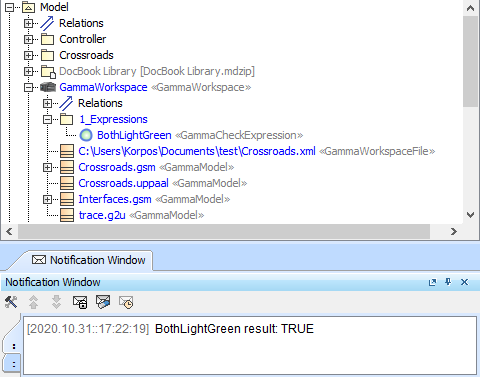
\includegraphics[width=10cm, keepaspectratio]{figures/contribution/verif1.png}
	\caption{Verifikáció futtatásának eredménye}
	\label{fig:verif1}
\end{figure}


Tehát a feltétel teljesül. Ezt az eredményt nem kielégítő hiszen azt szeretnénk, ha ez soha nem forduljon elő. Vizsgáljuk meg az példát amit kaptunk, hogy hogyan jutottunk el ebbe az állapotba (\ref{fig:trace-signals} ábra). A végrehajtás a harmadik lépésig a megszokott viselkedést produkálja azonban a negyedik lépésben érkezik egy \emph{police} szignál. Ennek határára a negyedik lépésben a két lámpa \emph{Interrupted} állapotba vált. Ugyan ebben a lépésben érkezik még egy \emph{police} szignál. Ezután az ötödik lépésben már hibás állapotba kerül a rendszer. Ennek az oka talán elsőre nem annyira látszik, de ha közelebbről megvizsgáljuk az állapotokat azt láthatjuk, hogy a  harmadik, negyedik és ötödik lépésben is a \emph{controller} a \emph{Secondary} állapotba lép bele. Ennek az állapot belépéskor végrehajtja a \emph{toggleBoth} (\ref{fig:activity} ábra) viselkedést, ami először a \emph{priority} majd a \emph{secondary} partoknak küldi el a \emph{toggle} szignálokat ebben a sorrendben. A negyedik lépésben \emph{primary} piros a \emph{secodnary} épp zöld így amikor a következő lépésben megérkezik előbb a \emph{primary}ba a \emph{toggle} szignál, így ő átlép a zöldbe még mielőtt a \emph{secondary} váltana így teljesül a tulajdonság.

\begin{figure}[!ht]
	\centering
	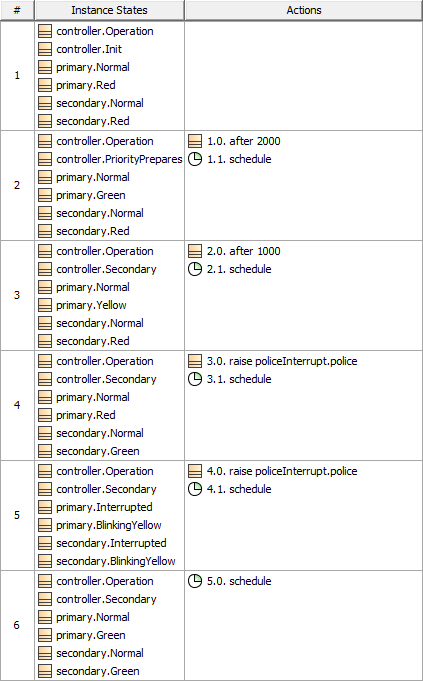
\includegraphics[width=10cm, keepaspectratio]{figures/contribution/traces_example.png}
	\caption{Verifikáció futtatásának eredménye}
	\label{fig:traces-example}
\end{figure}


\newpage
\section{Modell javítása}

A problémát úgy lehet kiküszöbölni talán a legkönnyebben, hogy a \emph{Controller}-be is felveszünk egy olyan állapotot amikor várakozik (\ref{fig:fixed} ábra). így már nem történik meg a többször egymás utáni szignál elküldés. Legalább is ezt feltételezzük.

\begin{figure}[!ht]
	\centering
	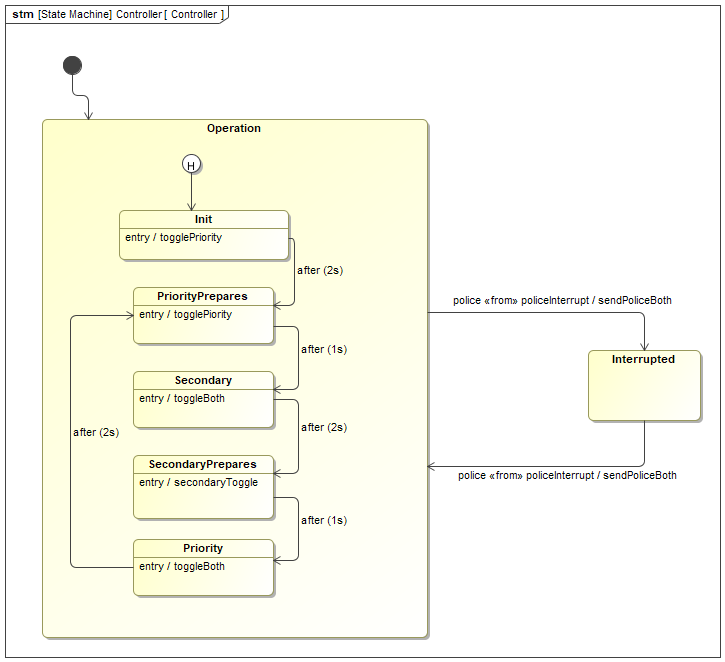
\includegraphics[width=10cm, keepaspectratio]{figures/contribution/ControllerFixed.png}
	\caption{Javított \emph{Controller} állapottérképe}
	\label{fig:fixed}
\end{figure}

A transzformációkat újra végre kell hajtani, hiszen a modell megváltozott. Viszont ha újra futtatjuk a verifikációt akkor már a tulajdonság nem lesz igaz, tehát valóban sikerült javítani a modellt (\ref{fig:verif2} ábra).

\begin{figure}[!ht]
	\centering
	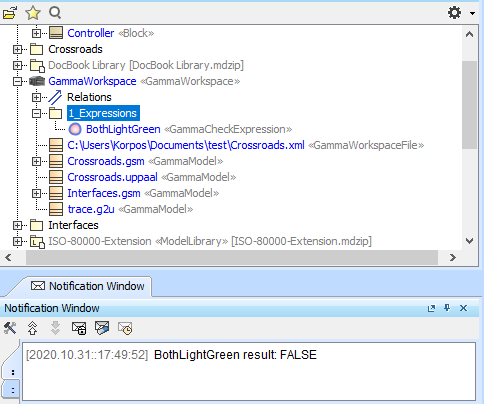
\includegraphics[width=10cm, keepaspectratio]{figures/contribution/verif2.png}
	\caption{Verifikáció futtatásának eredménye a javított modellen}
	\label{fig:verif2}
\end{figure}